% Capítulo 2: compilação, interpretação e o caminho híbrido do Java.
\documentclass[border=4pt]{standalone}
\usepackage[utf8]{inputenc}
\usepackage[T1]{fontenc}
% Estilo comum dos fluxogramas e diagramas de blocos.
\usepackage{tikz}
\usetikzlibrary{arrows.meta, positioning, calc, shapes.geometric, shapes.misc}
\definecolor{navy}{RGB}{23,45,80}
\definecolor{laranja}{RGB}{250,110,29}
\definecolor{cinzalogo}{RGB}{107,114,126}
\definecolor{azul}{RGB}{205,222,247}
\tikzset{
  base/.style={draw=navy, line width=0.9pt, font=\sffamily\small, align=center, inner sep=4pt},
  terminal/.style={base, rounded rectangle, fill=laranja!45, draw=laranja, minimum width=20mm, minimum height=7mm},
  processo/.style={base, rectangle, fill=laranja!12, minimum width=28mm, minimum height=8mm},
  decisao/.style={base, diamond, aspect=2.2, fill=azul, inner sep=1pt, minimum width=30mm},
  es/.style={base, trapezium, trapezium left angle=72, trapezium right angle=108,
             fill=white, minimum width=26mm, minimum height=8mm, trapezium stretches body},
  fluxo/.style={-{Stealth[length=2.2mm]}, navy, line width=0.9pt},
  rotulo/.style={font=\sffamily\small\bfseries, text=navy},
  legenda/.style={font=\sffamily\scriptsize, text=cinzalogo},
  resposta/.style={font=\sffamily\scriptsize\bfseries, text=navy},
}

\tikzset{
  arquivo/.style={base, rectangle, fill=white, minimum width=20mm, minimum height=8mm, font=\ttfamily\scriptsize},
  etapa/.style={base, rectangle, rounded corners=3pt, fill=laranja!12, minimum width=22mm, minimum height=8mm, font=\sffamily\scriptsize},
  final/.style={base, rectangle, rounded corners=3pt, fill=azul, minimum width=22mm, minimum height=8mm, font=\sffamily\scriptsize},
  linguagem/.style={font=\sffamily\small\bfseries, text=navy, anchor=east},
  quando/.style={font=\sffamily\scriptsize, text=laranja},
}
\begin{document}
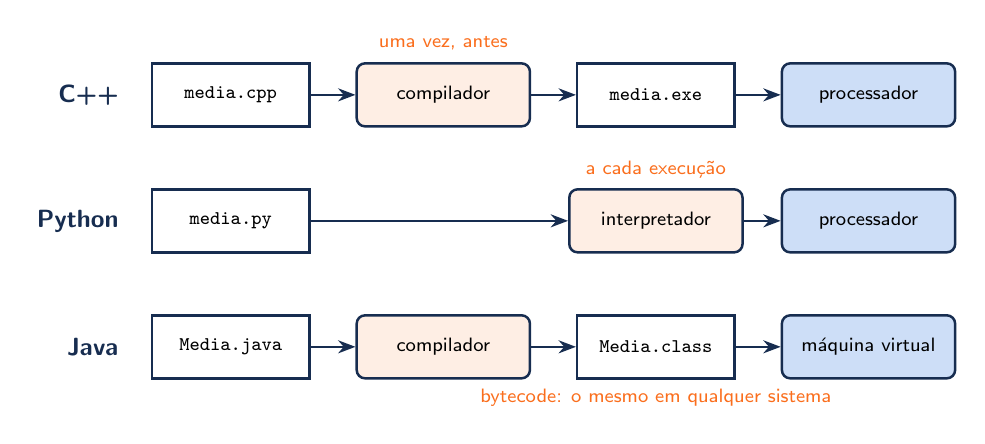
\begin{tikzpicture}
  % compilada
  \node[linguagem] at (-0.4, 0) {C++};
  \node[arquivo] (a1) at (0.9, 0) {media.cpp};
  \node[etapa] (b1) at (3.6, 0) {compilador};
  \node[arquivo] (c1) at (6.3, 0) {media.exe};
  \node[final] (d1) at (9.0, 0) {processador};
  \draw[fluxo] (a1) -- (b1);
  \draw[fluxo] (b1) -- (c1);
  \draw[fluxo] (c1) -- (d1);
  \node[quando] at (3.6, 0.65) {uma vez, antes};

  % interpretada
  \node[linguagem] at (-0.4, -1.6) {Python};
  \node[arquivo] (a2) at (0.9, -1.6) {media.py};
  \node[etapa] (b2) at (6.3, -1.6) {interpretador};
  \node[final] (d2) at (9.0, -1.6) {processador};
  \draw[fluxo] (a2) -- (b2);
  \draw[fluxo] (b2) -- (d2);
  \node[quando] at (6.3, -0.95) {a cada execução};

  % híbrida
  \node[linguagem] at (-0.4, -3.2) {Java};
  \node[arquivo] (a3) at (0.9, -3.2) {Media.java};
  \node[etapa] (b3) at (3.6, -3.2) {compilador};
  \node[arquivo] (c3) at (6.3, -3.2) {Media.class};
  \node[final] (d3) at (9.0, -3.2) {máquina virtual};
  \draw[fluxo] (a3) -- (b3);
  \draw[fluxo] (b3) -- (c3);
  \draw[fluxo] (c3) -- (d3);
  \node[quando] at (6.3, -3.85) {bytecode: o mesmo em qualquer sistema};
\end{tikzpicture}
\end{document}
